\chapterheading{1}{GIỚI THIỆU ĐỀ TÀI}
\setcounter{section}{1}
\setcounter{subsection}{0}
\setcounter{subsubsection}{0}

\subsection{Bối cảnh và vấn đề nghiên cứu}
Các hệ thống chấm công bằng thẻ, vân tay hoặc nhận diện khuôn mặt tại cửa thường ghi nhận tốt các mốc vào/ra, nhưng không trực tiếp phản ánh việc một người có hiện diện tại khu vực làm việc trong khoảng thời gian giữa hai mốc đó hay không. Trong môi trường có nhiều bàn làm việc và camera giám sát cố định, video cung cấp một nguồn quan sát liên tục có thể được chuyển thành các khoảng hiện diện. Tuy nhiên, việc chuyển dữ liệu video thành đại lượng thời gian tin cậy đòi hỏi nhiều bước hơn một phép phát hiện người đơn lẻ.

Từ góc nhìn thị giác máy tính, một detector có thể bỏ sót người trong vài khung hình do che khuất, chuyển động nhanh, độ phân giải thấp hoặc ánh sáng thay đổi. Nếu hệ thống cộng thời gian dựa trực tiếp trên từng frame, các lỗi ngắn sẽ tạo thành nhiều đoạn hiện diện bị ngắt quãng và gây sai số tích lũy. Ngược lại, nếu duy trì trạng thái quá lâu sau khi mất detection thì hệ thống có thể tính cả thời gian người đã rời khỏi vùng. Vì vậy, bài toán cần đồng thời kết hợp phát hiện, theo dõi đa đối tượng, hình học vùng quan tâm và xử lý tín hiệu theo thời gian.

Một khó khăn khác là khung hình CCTV có thể chứa nhiều nhân viên. Detection ở frame hiện tại không mang theo danh tính từ frame trước. Thuật toán theo dõi đa đối tượng phải gán một track ID tạm thời cho mỗi người, duy trì quỹ đạo và hạn chế đổi ID. SORT đã chứng minh một pipeline theo dõi trực tuyến có thể đạt tốc độ cao bằng Kalman filter và Hungarian assignment \cite{sort}; Deep SORT bổ sung đặc trưng ngoại hình nhằm giảm identity switch khi che khuất \cite{deepsort}; ByteTrack tiếp tục cải thiện hướng tracking-by-detection bằng cách liên kết cả detection có điểm tin cậy thấp để phục hồi track bị suy giảm do che khuất \cite{bytetrack}. Đồ án chọn ByteTrack vì phù hợp với yêu cầu trực tuyến và có thể tích hợp trực tiếp với đầu ra detector.

Ngoài việc ghi nhận hiện diện, yêu cầu bổ sung của đề tài là theo dõi thời gian sử dụng điện thoại. Đây không thể được mô hình hóa đơn giản bằng quy tắc ``frame có cell phone thì nhân viên đang dùng điện thoại'', bởi điện thoại có thể nằm trên bàn, thuộc người khác hoặc chỉ xuất hiện trong vài khung hình. Hệ thống cần liên kết detection điện thoại với track người theo quan hệ không gian, sau đó xác nhận một phiên sử dụng bằng điều kiện thời gian. Tổng thời gian sử dụng được so sánh với hạn mức cấu hình; chỉ phần vượt hạn mức mới tham gia phép điều chỉnh thời gian làm việc.

Trong đồ án này, cụm từ \textit{thời gian làm việc} được định nghĩa vận hành là \textbf{thời gian hiện diện ước lượng trong khu vực làm việc, sau khi áp dụng chính sách trừ phần thời gian sử dụng điện thoại vượt mức cho phép}. Định nghĩa này không đồng nghĩa với năng suất, mức độ tập trung, kết quả công việc hay thời gian lao động pháp lý. Việc phân biệt khái niệm giúp giới hạn đúng phạm vi khoa học của hệ thống và tránh diễn giải quá mức từ dữ liệu hình ảnh.

\subsection{Mục tiêu nghiên cứu}
\subsubsection{Mục tiêu tổng quát}
Mục tiêu tổng quát là xây dựng một hệ thống thị giác máy tính có khả năng quan sát đồng thời nhiều nhân viên từ một camera CCTV cố định, xác định trạng thái hiện diện của từng nhân viên trong khu vực làm việc, theo dõi thời lượng sử dụng điện thoại, ước lượng thời gian làm việc theo chính sách và cung cấp dữ liệu gần thời gian thực cho hệ thống quản trị, hậu kiểm và báo cáo.

\subsubsection{Mục tiêu cụ thể}
Đồ án đặt ra các mục tiêu cụ thể sau:
\begin{itemize}
\item Phát hiện đồng thời lớp \textit{person} và \textit{cell phone} từ cùng một khung hình bằng YOLOv8, tránh chạy lặp detector cho từng chức năng.
\item Tích hợp ByteTrack để duy trì track ID của nhiều người qua thời gian và giảm phân mảnh quỹ đạo trong các đoạn che khuất ngắn.
\item Cho phép cấu hình một hoặc nhiều vùng làm việc dạng đa giác trên ảnh camera, gán vùng với nhân viên hoặc vị trí công việc và xác định quan hệ người--vùng bằng điểm neo ở đáy bounding box.
\item Tận dụng face embedding để hỗ trợ xác minh rằng track trong vùng phù hợp với nhân viên được gán, nhưng không phụ thuộc vào nhận diện khuôn mặt ở mọi frame.
\item Thiết kế máy trạng thái hiện diện gồm các trạng thái trung gian để lọc bỏ detection miss ngắn, đồng thời lưu chính xác mốc bắt đầu/kết thúc khoảng hiện diện.
\item Thiết kế máy trạng thái sử dụng điện thoại và thuật toán liên kết phone--person nhằm tránh gán một điện thoại cho nhiều nhân viên hoặc coi điện thoại đặt trên bàn là đang sử dụng.
\item Xây dựng bộ tổng hợp thời gian tạo các \textit{presence interval}, tính tổng hiện diện, tổng thời gian điện thoại, phần vượt mức cho phép và thời gian làm việc hiệu lực.
\item Xây dựng backend FastAPI, WebSocket, cơ sở dữ liệu quan hệ, kho bằng chứng, phân quyền và dashboard theo dõi theo thời gian thực.
\item Thiết kế quy trình đánh giá gồm chỉ số detection, tracking, presence F1, phone-use F1, sai số gán điện thoại, MAE/MAPE thời gian và hiệu năng xử lý.
\item Thiết kế hệ thống theo nguyên tắc tối thiểu hóa dữ liệu, truy vết được và có chính sách lưu trữ phù hợp với yêu cầu bảo vệ dữ liệu cá nhân.
\end{itemize}

\subsection{Đối tượng và phạm vi nghiên cứu}
\subsubsection{Đối tượng nghiên cứu}
Đối tượng nghiên cứu gồm các phương pháp phát hiện đối tượng trong video, theo dõi đa đối tượng, face embedding, hình học ROI, xử lý tín hiệu thời gian, tổng hợp khoảng hiện diện, phát hiện phiên sử dụng điện thoại, kiến trúc giao tiếp thời gian thực và mô hình dữ liệu phục vụ giám sát nhiều nhân viên.

Đồ án không nghiên cứu nội dung công việc mà nhân viên đang thực hiện, không phân tích bàn phím/màn hình, không nhận dạng nội dung điện thoại, không nghe âm thanh và không sử dụng mô hình để suy luận cảm xúc, thái độ hoặc năng suất cá nhân.

\subsubsection{Phạm vi thực hiện}
Phạm vi kỹ thuật được xác định như sau:
\begin{itemize}
\item Một camera CCTV cố định quan sát đồng thời nhiều vị trí làm việc trong cùng không gian.
\item Video được xử lý theo thời gian gần thực; đầu vào có thể là RTSP, tệp video hoặc webcam trong môi trường phát triển.
\item YOLOv8n hoặc một biến thể cùng họ được dùng cho lớp người và điện thoại; model có thể được thay bằng weight fine-tune nếu có dữ liệu thực địa nhưng kiến trúc hệ thống không phụ thuộc vào một weight cụ thể.
\item ByteTrack được dùng làm tracker chính; track ID chỉ là định danh tạm thời của quỹ đạo.
\item Khu vực làm việc được quản trị viên vẽ bằng polygon trên ảnh tham chiếu của camera.
\item FaceNet embedding là tín hiệu xác minh hỗ trợ. Nếu khuôn mặt quá nhỏ, quay lệch hoặc bị che, hệ thống chuyển trạng thái identity sang \textit{unknown/provisional} thay vì ép kết luận.
\item Hạn mức điện thoại được cấu hình theo ca hoặc theo tổ chức. Chỉ thời gian vượt hạn mức mới được trừ khỏi thời gian hiện diện.
\item Backend hỗ trợ tổ chức, người dùng quản trị, nhân viên, camera, khu vực, chính sách, phiên giám sát, sự kiện, báo cáo và nhật ký kiểm toán.
\item Hệ thống không tự động đưa ra quyết định kỷ luật. Dữ liệu được trình bày như bằng chứng hỗ trợ con người xem xét.
\end{itemize}

\subsubsection{Nội dung ngoài phạm vi}
Các nội dung sau được đặt ngoài phạm vi của phiên bản đồ án:
\begin{itemize}
\item Nhận diện xuyên camera giữa nhiều camera chưa đồng bộ hình học.
\item Re-identification toàn thân ở quy mô lớn khi nhân viên thay đổi quần áo hoặc xuất hiện ở nhiều ngày khác nhau.
\item Suy luận hành vi ``làm việc/chơi'' từ tư thế, biểu cảm hoặc nội dung màn hình.
\item Xác định chính xác người đang cầm điện thoại trong mọi trường hợp tay và điện thoại bị che hoàn toàn.
\item Chống giả mạo sinh trắc học chuyên dụng hoặc nhận diện deepfake.
\item Tự động áp dụng chế tài nhân sự dựa trên kết quả mô hình.
\item Khẳng định độ chính xác triển khai thực tế khi chưa thay số liệu mô phỏng bằng dữ liệu CCTV có ground truth.
\end{itemize}

\subsection{Bài toán ước lượng thời gian làm việc}
Tại thời điểm $t$, xét tập detection người $D_t=\{d_t^1,\ldots,d_t^n\}$. Tracker biến chuỗi detection thành tập track $Q_t=\{q_t^1,\ldots,q_t^m\}$, mỗi track có bounding box, độ tin cậy và track ID. Với một vùng làm việc $A_e$ gán cho nhân viên $e$, hệ thống tính điểm neo của track $q$:
\begin{equation}
 p(q)=\left(\frac{x_1+x_2}{2},y_2\right),
 \label{eq:anchor}
\end{equation}
trong đó $(x_1,y_1,x_2,y_2)$ là bounding box. Track là ứng viên của vùng nếu $p(q)\in A_e$. Việc dùng điểm đáy thay cho tâm hộp giúp xấp xỉ tốt hơn vị trí người trên mặt phẳng sàn khi bounding box cao và giao nhau.

Sau khi liên kết không gian, máy trạng thái biến chuỗi quan sát nhị phân thành các khoảng hiện diện $I_e=\{[s_k,e_k]\}$. Tổng thời gian hiện diện trong cửa sổ đánh giá $W$ là:
\begin{equation}
 T_{presence}(e)=\sum_k |[s_k,e_k]\cap W|.
 \label{eq:presence}
\end{equation}
Tương tự, các phiên sử dụng điện thoại đã xác nhận tạo thành tập $P_e$. Tổng thời gian sử dụng điện thoại chỉ được tính trên phần giao với khoảng hiện diện và lịch làm việc:
\begin{equation}
 T_{phone}(e)=\sum_j |P_j\cap I_e\cap W|.
 \label{eq:phone}
\end{equation}
Với hạn mức $T_{allow}$, phần vượt mức là:
\begin{equation}
 T_{excess}(e)=\max(0,T_{phone}(e)-T_{allow}).
 \label{eq:excess}
\end{equation}
Thời gian làm việc hiệu lực được định nghĩa:
\begin{equation}
 T_{effective}(e)=\max(0,T_{presence}(e)-T_{excess}(e)).
 \label{eq:effective}
\end{equation}
Cách tách bốn đại lượng ở trên giúp bảo toàn dữ liệu gốc và cho phép giải thích đầy đủ mọi điều chỉnh.

\subsection{Định hướng giải pháp}
Giải pháp được tổ chức theo năm lớp trách nhiệm. Lớp thu nhận nhận frame từ CCTV và chuẩn hóa kích thước. Lớp nhận thức chạy YOLOv8 một lần để tạo detection người và điện thoại. Lớp theo dõi dùng ByteTrack duy trì quỹ đạo người. Lớp ngữ cảnh thực hiện ROI matching, liên kết identity và phone--person. Lớp thời gian cập nhật máy trạng thái hiện diện/điện thoại, sinh event và tổng hợp thời lượng. Kết quả được đẩy lên backend theo WebSocket; server lưu current state trong SQL để dashboard tải nhanh và lưu event/ảnh bằng chứng theo dòng thời gian để hậu kiểm.

\begin{figure}[H]
\centering
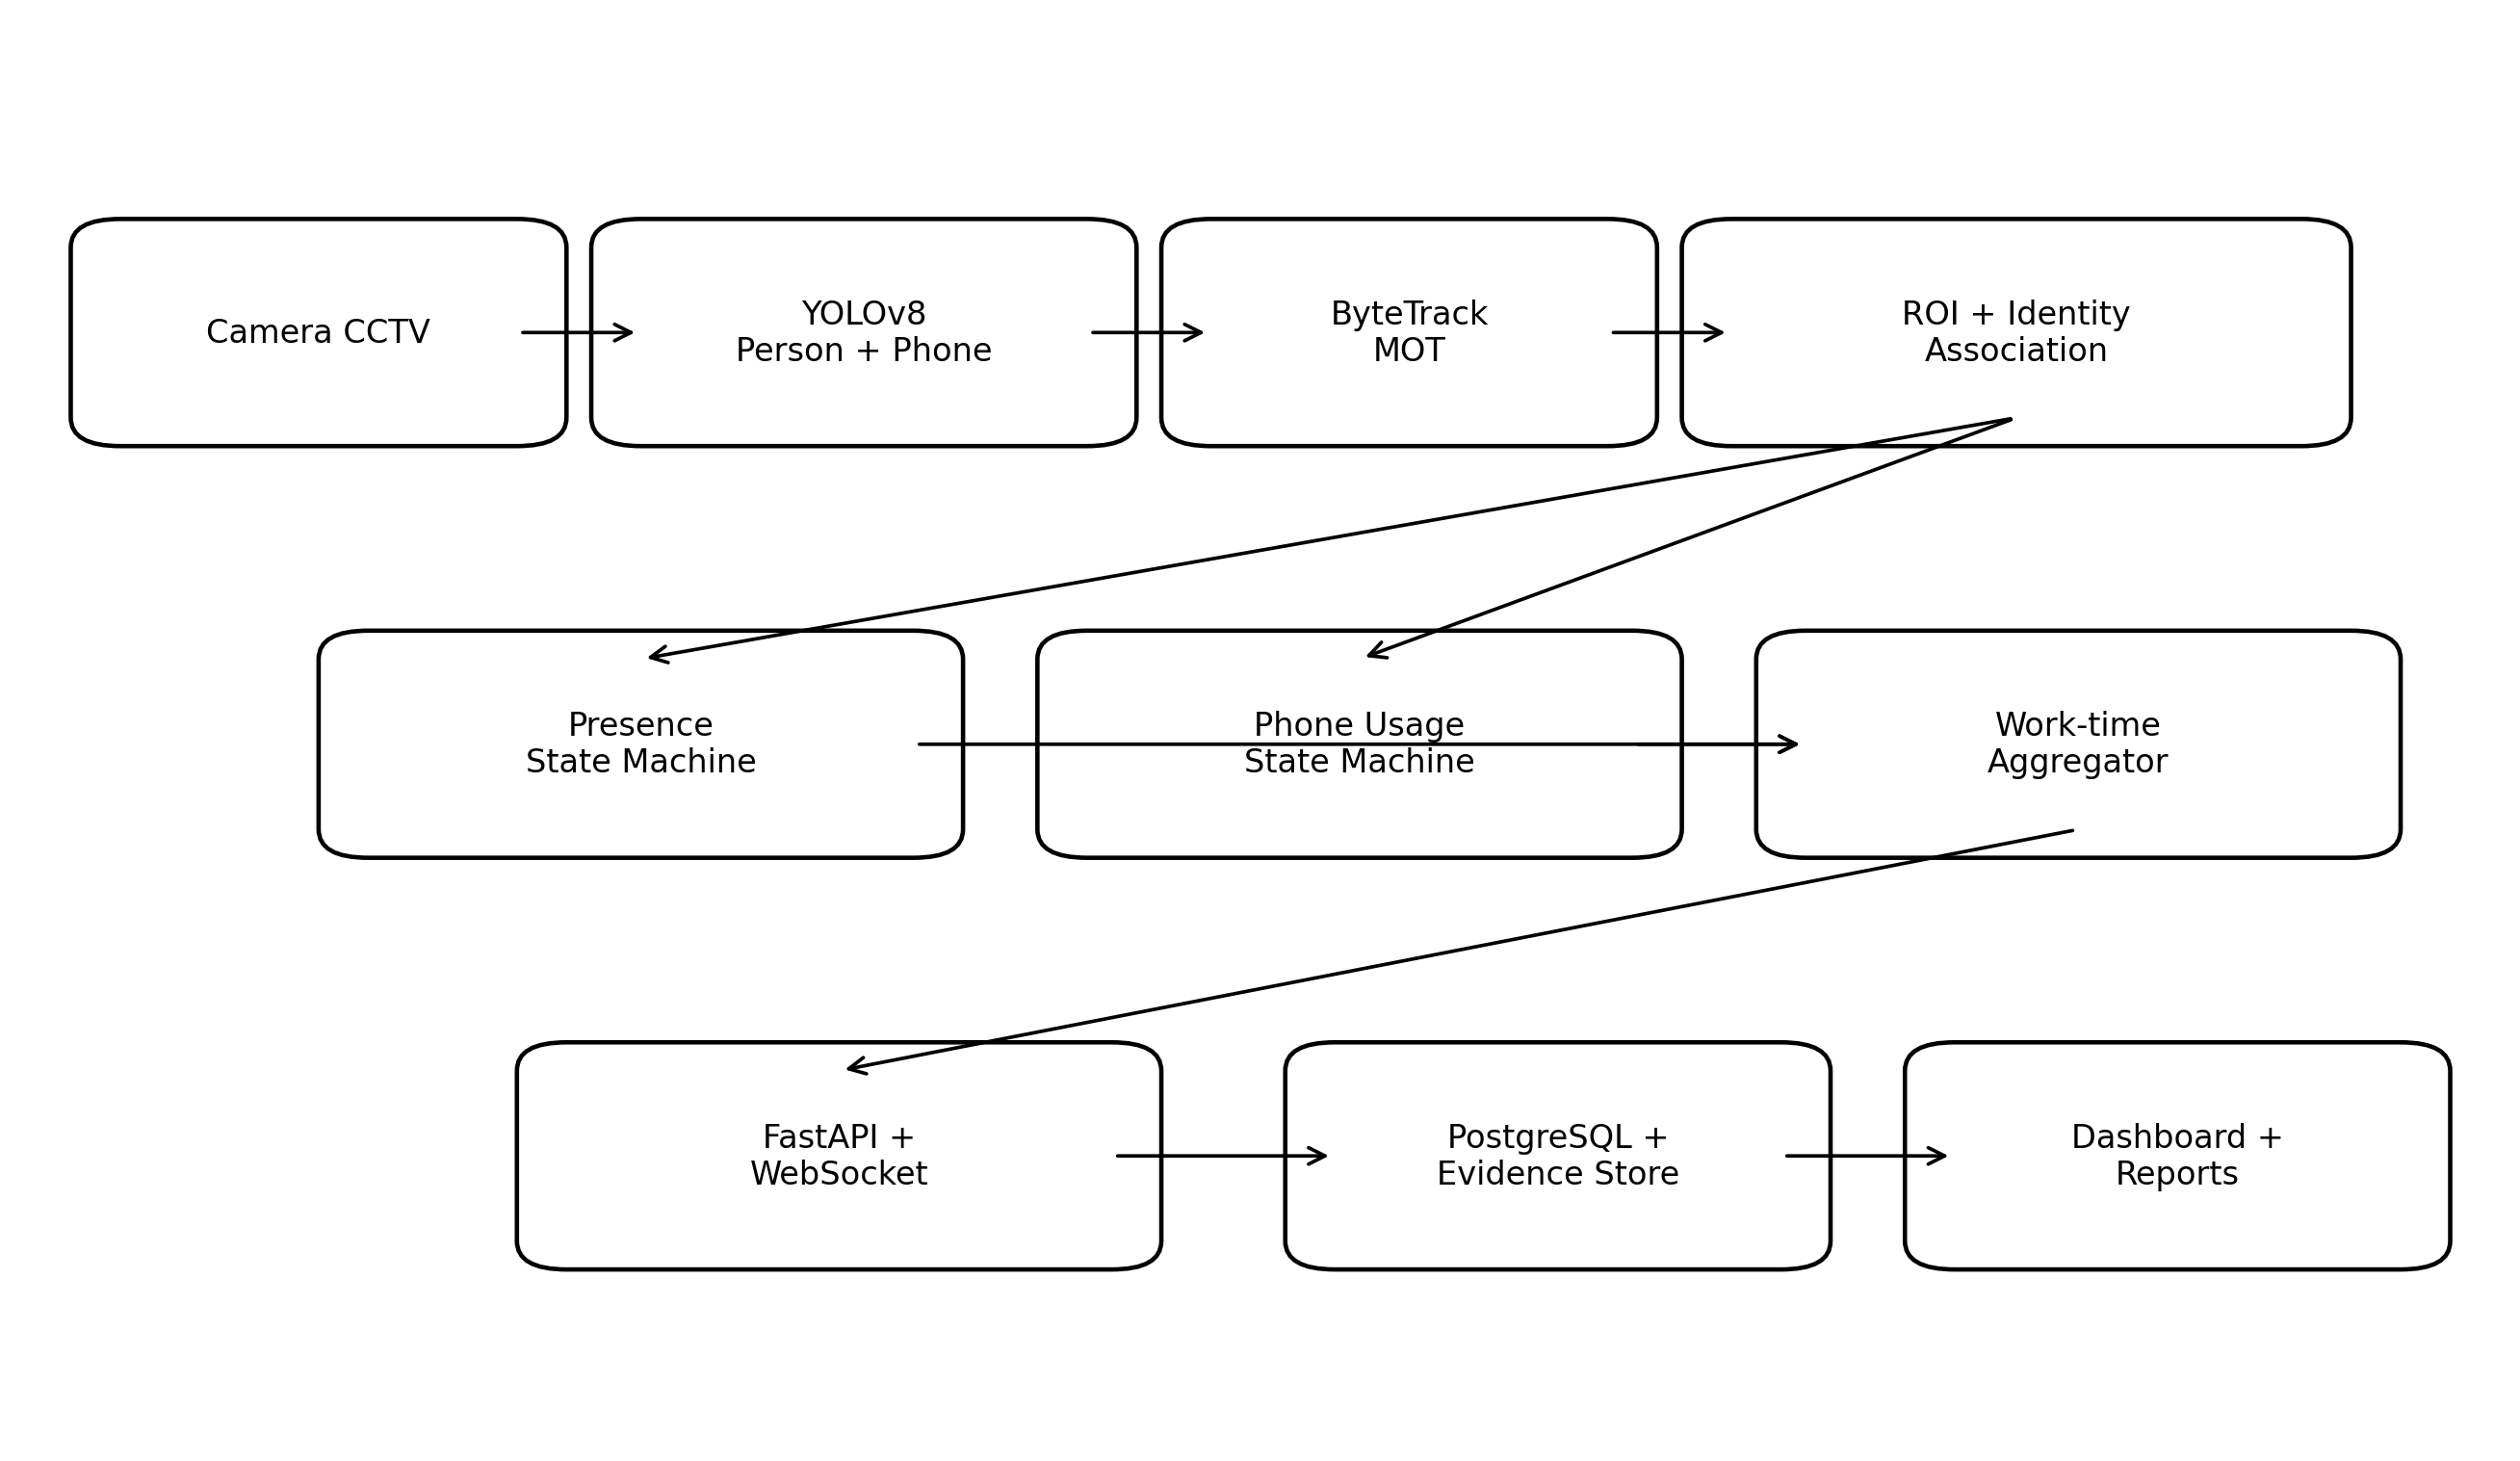
\includegraphics[width=0.96\textwidth]{Images/new_architecture.png}
\caption{Kiến trúc tổng thể của hệ thống đề xuất}
\label{fig:overall-architecture}
\end{figure}

Kiến trúc này duy trì nguyên tắc ``một lần nhận thức, nhiều bộ xử lý sử dụng chung kết quả''. YOLO không được chạy riêng cho person và phone; thay vào đó một kết quả suy luận được tách theo lớp. Face verification cũng không chạy mọi frame mà chỉ kích hoạt theo sự kiện: track mới, identity chưa đủ chắc chắn hoặc đến chu kỳ kiểm tra. Điều này giúp giảm tải và giảm phụ thuộc vào chất lượng khuôn mặt liên tục.

\subsection{Các đóng góp chính}
Các đóng góp kỹ thuật và hệ thống của đồ án gồm:
\begin{enumerate}
\item Kiến trúc camera đa người kết hợp detector, tracker và polygon ROI để chuyển video thành chuỗi hiện diện theo từng nhân viên.
\item Cơ chế liên kết định danh theo hai tầng: vị trí/ROI là tín hiệu duy trì chính, face embedding là tín hiệu xác minh khi đủ chất lượng; trạng thái không chắc chắn được biểu diễn tường minh thay vì ép nhãn.
\item Máy trạng thái hiện diện có khoảng đệm, cho phép hấp thụ detection miss ngắn nhưng vẫn truy hồi thời điểm bắt đầu/kết thúc thật để hạn chế sai số thời gian có hệ thống.
\item Cơ chế liên kết phone--person và máy trạng thái sử dụng điện thoại, chỉ tính phiên sử dụng khi detection liên quan đúng track và duy trì đủ lâu.
\item Mô hình tổng hợp thời gian tách gross presence, phone usage, allowance, excess và effective work time để bảo đảm khả năng giải thích.
\item Nền tảng backend nhiều tổ chức với WebSocket, RBAC, evidence store, report job và audit log, cho phép giám sát nhiều nhân viên trong cùng camera mà không cần truyền toàn bộ video đến dashboard.
\item Khung đánh giá đa tầng kết nối chất lượng detection/tracking với sai số cuối cùng theo đơn vị thời gian, thay vì chỉ báo cáo Accuracy/F1 ở cấp frame.
\end{enumerate}

\subsection{Bố cục báo cáo}
Chương 2 trình bày cơ sở lý thuyết về object detection, YOLOv8, tracking-by-detection, ByteTrack, ROI, FaceNet, xử lý thời gian, phát hiện sử dụng điện thoại và các chỉ số đánh giá. Chương 3 khảo sát phương án chấm công và phân tích yêu cầu. Chương 4 mô tả thiết kế hệ thống, state machine, mô hình dữ liệu và luồng thời gian. Chương 5 trình bày cài đặt dự kiến từ mã nguồn nền hiện có. Chương 6 xây dựng quy trình kiểm thử và minh họa bằng dữ liệu mô phỏng có ghi nhãn rõ. Chương 7 tổng kết kết quả thiết kế, hạn chế và hướng phát triển.
